

\documentclass{article}
\usepackage{times,amsmath,amsthm,amsfonts,eucal,graphicx}
\usepackage{float}
\usepackage{algorithm}
\usepackage[noend]{algpseudocode}
\usepackage{hyperref}

\algrenewcommand\alglinenumber[1]{\footnotesize #1}
\algblock[Name]{Struct}{End}

\usepackage{tikz}
\usetikzlibrary{arrows,shapes,positioning}
\usetikzlibrary{decorations.markings}
\tikzstyle arrowstyle=[scale=1]
\tikzstyle directed=[postaction={decorate,decoration={markings,
mark=at position .6 with {\arrow[arrowstyle]{stealth}}}}]

\setlength{\oddsidemargin}{0.25 in}
\setlength{\evensidemargin}{-0.25 in}
\setlength{\topmargin}{-0.6 in}
\setlength{\textwidth}{6.5 in}
\setlength{\textheight}{8.5 in}
\setlength{\headsep}{0.75 in}
\setlength{\parindent}{0 in}
\setlength{\parskip}{0.1 in}

\newcounter{lecnum}
\renewcommand{\thepage}{\thelecnum-\arabic{page}}
\renewcommand{\thesection}{\thelecnum.\arabic{section}}
\renewcommand{\theequation}{\thelecnum.\arabic{equation}}
\renewcommand{\thefigure}{\thelecnum.\arabic{figure}}
\renewcommand{\thetable}{\thelecnum.\arabic{table}}

%
\newcommand{\indep}{{\bot\negthickspace\negthickspace\bot}}
\newcommand{\notindep}{{\not\negthickspace\negthinspace{\bot\negthickspace\negthickspace\bot}}}
\newcommand{\definedtobe}{\stackrel{\Delta}{=}}
\renewcommand{\choose}[2]{{{#1}\atopwithdelims(){#2}}}
\newcommand{\argmax}[1]{{\hbox{$\underset{#1}{\mbox{argmax}}\;$}}}
\newcommand{\argmin}[1]{{\hbox{$\underset{#1}{\mbox{argmin}}\;$}}}

\newcommand{\lecture}[4]{
   \pagestyle{myheadings}
   \thispagestyle{plain}
   \newpage
   \setcounter{lecnum}{#1}
   \setcounter{page}{1}
   \noindent
   \begin{center}
   \framebox{
      \vbox{\vspace{2mm}
    \hbox to 6.58in { {\bf [CS252]-Algorithms II
                        \hfill Spring 2021-22} }
    \hbox to 6.58in { {\bf 
                        \hfill } }
       \vspace{4mm}
       \hbox to 6.28in { {\Large \hfill Homework: 02 \hfill} }
       \vspace{2mm}
       \hbox to 2.28in { { Name: Sudhir Sharma   \hspace{2cm} RollNo: 12041500 \hspace{2cm} email: sudhirsharma@iitbhlai.ac.in} }
      \vspace{5mm}
  \hbox to 1.0in { { Collaborators Names:    } }
  
}
   }
   \end{center}

   \vspace*{4mm}
}

\renewcommand{\cite}[1]{[#1]}
\def\beginrefs{\begin{list}%
        {[\arabic{equation}]}{\usecounter{equation}
         \setlength{\leftmargin}{2.0truecm}\setlength{\labelsep}{0.4truecm}%
         \setlength{\labelwidth}{1.6truecm}}}
\def\endrefs{\end{list}}
\def\bibentry#1{\item[\hbox{[#1]}]}

\newcommand{\fig}[4]{
			\begin{center}
	                \includegraphics[width=#4,clip=true]{#3} \\
			Figure \thelecnum.#1:~#2
			\end{center}
	}

\theoremstyle{definition}
% Use these for theorems, lemmas, proofs, etc.
\newtheorem{theorem}{Theorem}[lecnum]
\newtheorem{lemma}[theorem]{Lemma}
\newtheorem{proposition}[theorem]{Proposition}
\newtheorem{claim}[theorem]{Claim}
\newtheorem{corollary}[theorem]{Corollary}
\newtheorem{definition}[theorem]{Definition}
\newtheorem{problem}{Solution of problem}

% \newenvironment{proof}{{\bf Proof:}}{\hfill\rule{2mm}{2mm}}

% **** IF YOU WANT TO DEFINE ADDITIONAL MACROS FOR YOURSELF, PUT THEM HERE:

\begin{document}
%FILL IN THE RIGHT INFO.
%\lecture{**LECTURE-NUMBER**}{**DATE**}{**LECTURER**}{**SCRIBE**}
\lecture{1}{}{xxx}


% **** YOUR NOTES GO HERE:
\begin{problem}
	\hspace{2cm}\\
  \textbf{Forward:}

  We know that if a Graph $G$ has no negative cycles, then there is a shortest path from $s$ to $t$ that is simple (no cycles) and hence have at most $n-1$ edges. This means that if there are no negative cycles in $G$, then $opt(i,v) = opt(n-1,v)$ for all vertices $v$ and for all $i\geq n$.\\
  \textbf{Backward:}

  Suppose  $opt(n,v) = opt(n-1,v)$ for all $v\in V$

  \begin{eqnarray*}
    opt(n,v) &=& \min\left(opt(n-1,v), \min_{u\in E}\left(opt(n-1,u)+w_{u,v}\right)\right)\\
    \implies opt(n,v) &\leq& opt(n-1,u)+w_{u,v} ~~\forall ~~u\in E\\
    \implies w_{u,v} &\geq& opt(n,v) - opt(n-1,u)
  \end{eqnarray*}
  Let $C$ be any arbitrary cycle.
  \begin{eqnarray*}
    \sum_{(u,v)\in C} w_{u,v} \geq \sum_{(u,v)\in C}(opt(n,v) -opt(n-1,u)) = 0
  \end{eqnarray*}
  Therefore, there does not exist any negative weight cycle.

  The below figure is the Bellman-Ford algorithm for no negative edge weight cycle.
  \begin{figure}[h!]
    \centering
    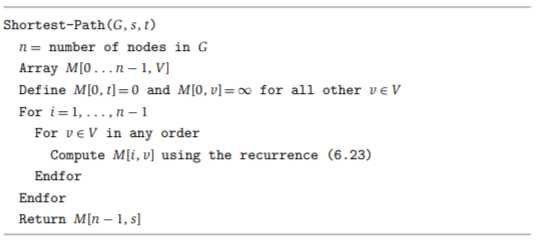
\includegraphics{bellman.PNG}
  \end{figure}
  We can create the matrix $M$ of size $(0\dots n,V)$ instead of $(0\dots n-1,V)$. We can run the outermost for loop for $n$ times instead of $n-1$ times.
  After the end of algorithm and before the return statement, we can include a for loop to check whether $M[n][v] = M[n-1][v]~~\forall~~v\in V$. If not, then there exists a negative weight cycle.

  Below is the modified Bellman-Ford Algorithm.

  \begin{algorithm}[H]
    \caption{Bellman-Ford Modified Algorithm}\label{}
    \begin{algorithmic}[1]
      \Procedure{bellman-ford-modified}{$G,s,t$}
      \State $n$ = number of nodes in $G$
      \State Array $M[0\dots n,V]$\Comment{$n+1$ rows}
      \State Define $M[0,t]=0$ and $M[0,v]= \infty$ for all other $v\in V$
      \For{$i\gets 1,n$} \Comment{Run till $n$}
        \For{$v\in V$}
          \State $M(i,v) = \min\left(M(i-1,v), \min_{u\in E}(M(i-1,u)+w_{u,v})\right)$
        \EndFor
      \EndFor
      \For{$v\in V$} \Comment{Check for negative weight cycle}
        \If{$M[n][v] \not = M[n-1][v]$}
          \State \textbf{return} $True,M[n-1,s]$\Comment{Return true i.e. negative cycle exists and $M[n-1,s]$}
        \EndIf
      \EndFor
      \State \textbf{return} $False,M[n-1,s]$\Comment{Return false i.e. negative cycle does not exists and $M[n-1,s]$}
      \EndProcedure
    \end{algorithmic}
  \end{algorithm}

\end{problem}
\begin{problem}
\hspace{2cm}\\
  \textbf{Backward:}

 Let $d_{ii}^{(n)}$ is the weight of the path from vertex $i$ to $i$. If $d_{ii}^{(n)} < 0$, it means that there is a path from $i$ to $i$ i.e a cycle of negative weight.

  \textbf{Forward:}

  Let $G$ has a negative weight cycle. Let $C$ be the mininum negative weight cycle out of all cycles. If $C$ has only one vertex (i.e. self loop), then $w_{ii} < 0$ so $d_{ii}^{k}$ for some $k$ starts negative and remains negative because $d_{ii}^{k}$ value is never increased in the algorithm. 

  If the cycle consists at least two vertices. Let $k$ be the highest numbered vertex in the cycle and $i$ be any other vertex in the cycle.  $d_{ik}^{(k-1)}$ and  $d_{ki}^{(k-1)}$ have the shortest paths weights because neither of them include the vertex $k$ as intermediate vertex and $i$ and $k$ are on $C$ which has the minimum negative weight. Since $i\rightarrow k \rightarrow i$ is a negative weight cycle, the sum of there weights becomes negative so  $d_{ii}^{(k)}$ becomes neagtive and its value is never increased in the algorithm. 
  
  The below figure is the Floyd-Warshall algorithm for no negative edge weight cycle.
  \begin{figure}[h!]
    \centering
    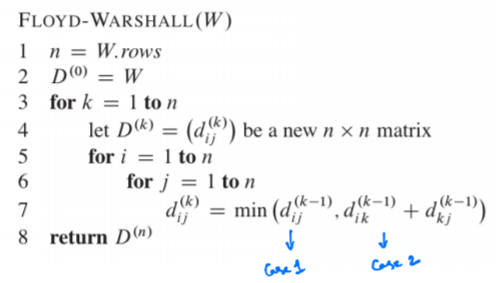
\includegraphics{floyd.PNG}
    \caption[]{Flyod Warshall Algorithm}
    \label{fig:Flyod}
  \end{figure}

  After line 7, in the above figure we can check weather the diagonal entries of matrix $D^{(n)}$. If any of the entry is negative, it means that the graph contains a negative weight cycle. If not, then the graph has no negative weight cycle. 

  Add the following loop After line 7 and before the return statement in \figurename{\ref{fig:Flyod}}.
  
  \begin{algorithm}[H]
    \caption{Floyd-Warshall updated}\label{}
    \begin{algorithmic}[1]
      \Procedure{Modification}{}
      \For{$i\gets 1,n$} \Comment{Check for diagonal entries of $D^{(n)}$}
        \If{$d_{ii}^{(n)} < 0$}
          \State \textbf{return} $False$
        \EndIf
      \EndFor
      \EndProcedure
    \end{algorithmic}
  \end{algorithm}

	\hspace{2cm}\\
	\textbf{Solution of Problem 3}\\
  (a) Value of the flow is sum of flow generated at source i.e. 4+4 = 8. This is not the maximum $s-t$ flow in this graph.
  
  (b) Residual graph
  \begin{center}
    \begin{tikzpicture}
      [scale = 0.65,auto=left]
      \node [circle,fill=gray!40](s) at (0,0) {$s$};
      \node [circle,fill=gray!40](v1) at (3,3) {$v_1$};
      \node [circle,fill=gray!40](v2) at (3,-3) {$v_2$};
      \node [circle,fill=gray!40](v3) at (8,3) {$v_3$};
      \node [circle,fill=gray!40](v4) at (8,-3) {$v_4$};
      \node [circle,fill=gray!40](t) at (11,0) {$t$};

      \draw[directed] (s) -- node[right]{12} (v1);
      \draw[directed] (v1) to [out=180,in=90] node[left]{4}  (s);
      \draw[directed] (v1) -- node{4} (v3);
      \draw[directed] (v3) to [out=135,in=45] node[above=4pt]{8} (v1);
      \draw[directed] (v3) -- node[below=2pt]{16} (t);
      \draw[directed] (t) to [out=90,in=0] node[above=4pt]{4} (v3);
      \draw[directed] (s) -- node{9} (v2);
      \draw[directed] (v2) to [out=180,in=-90] node{4} (s);
      \draw[directed] (v2) -- node{10} (v4);
      \draw[directed] (v4) to [out=225,in=-45] node{4} (v2);
      \draw[directed] (t) -- node{4} (v4);
      \draw[directed] (v1) -- node{4} (v2);
      \draw[directed] (v4) -- node{7} (v3);
      \draw[directed] (v3) -- node{5} (v2);
      \draw[directed] (v2) to [out=80,in=210] node{4} (v3);

    \end{tikzpicture}
  \end{center}

  (c) Value of the minimum $s-t$ cut is same as the max flow from $s-t$. $v(f) = 23$. Send 12 along edge $s-v_1$ and send 11 along edge $s-v_2$. The minimum cut can be $A =  \{s\}$ and $B = V-\{s\}$. The capacity of this cut is 16+13 = 29.

  
\end{problem}
% Some general latex examples and examples making use of the
% macros follow.  
%**** IN GENERAL, BE BRIEF AND COMPLETE. 

% **** THIS ENDS THE EXAMPLES. DON'T DELETE THE FOLLOWING LINE:

\end{document}


